%%%%%%%%%%%%%%%%%%%%%%%%%%%%%%%%%%%%%%%%%
%
% (c) 2022 by Jennifer Laaser
%
% This work is licensed under the Creative Commons Attribution-NonCommercial-ShareAlike 4.0 International License. To view a copy of this license, visit http://creativecommons.org/licenses/by-nc-sa/4.0/ or send a letter to Creative Commons, PO Box 1866, Mountain View, CA 94042, USA.
%
% The current source for these materials is accessible on Github: https://github.com/jlaaser/pogil-polymers
%
%%%%%%%%%%%%%%%%%%%%%%%%%%%%%%%%%%%%%%%%%

\renewcommand{\figpath}{content/polymphys/chain-confs/langevin-chains/figs}
\renewcommand{\labelbase}{langevin-chains}

\begin{activity}[extension]{Elasticity of Real Chains}
\label{\labelbase}

\begin{instructornotes}

	This activity introduces students to the force-extension curves of real chains, as exemplified by the Langevin chain model.
	
	After completing this activity, students will be able to:
			\begin{enumerate}
				\item Explain how strain-stiffening of polymer chains is related to their finite extensibility
				\item Use the Langevin model to calculate force-extension curves for freely-jointed polymer chains
				\item Identify the limits in which the Gaussian chain model is a good approximation for describing the force-extension behavior of polymer chains, and the limits in which it is not
			\end{enumerate}
	
			
	\subsection*{Activity summary:}
	\begin{itemize}
		\item \textbf{Activity type:} Learning Cycle
		\item \textbf{Content goals:} See above
		\item \textbf{Process goals:} %https://pogil.org/uploads/attachments/cj54b5yts006cklx4hh758htf-process-skills-official-pogil-list-2015-original.pdf
			\begin{itemize}
				\item Interpreting equations in terms of physical behavior
				\item Reading and interpreting graphs
				\item Oral and written communication of reasoning
			\end{itemize}
		\item \textbf{Duration:} approx. 30 min, including time for class discussion
		\item \textbf{Instructor preparation required:} 
			\begin{itemize}
				\item None beyond knowledge of relevant content
			\end{itemize}
		\item \textbf{Related textbook chapters:}
			\begin{itemize}
				\item \emph{Polymer Chemistry} (Hiemenz \& Lodge), 2nd ed.: not covered
				\item \emph{Introduction to Polymers} (Young \& Lovell), 3rd ed.: not covered
				\item \emph{Polymer Physics} (Rubinstein \& Colby): Section 2.6.2
				\item \emph{The Physics of Rubber Elasticity} (Treolar): Chapter 6
			\end{itemize}
	\end{itemize}

\end{instructornotes}

	%\textbf{Focus question:} Put a central question for the students to consider through this exercise here.


\begin{model}[Stretching a Chain to Near its Contour Length]
\label{\labelbase:model:chainstretching}

	A freely-jointed chain with 5 links of length $b$ is shown below:
	
	\vspace{6pt}
	\centerline{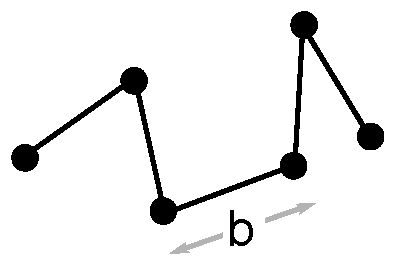
\includegraphics[width=0.3\textwidth]{\figpath/Model1_FJC.pdf}}

\end{model}

%\vspace{0.25in}
\begin{ctqs}

	\question Sketch the conformation of this chain in its fully extended state, e.g. when the two ends of the chain are as far away from each other as possible.  Assume the links are rigid and cannot stretch.
			
				\begin{solution}[0.25in]{}
					\centerline{
\includegraphics[width=0.5\textwidth]{\figpath/Model1_FJC_fullyextended_soln}}
				\end{solution}
			
	\question How long is this chain in its fully-extended state?
			
				\begin{solution}[0.25in]{}
					$5b$
				\end{solution}
			
	\question If the links are rigid and cannot stretch, is it physically possible for this chain to have an end-to-end distance longer than the value you calculated in part (b)?  Explain your group's reasoning in 1-2 complete sentences. \label{\labelbase:ctq:5b-reasoning}
			
				\begin{solution}[1.25in]{}
					No.  Once in this conformation, the chain cannot increase its end-to-end distance by further changes to the bond angles.  So, if the links are rigid and cannot stretch, it is not possible to draw a conformation in which the ends of the chain are farther apart.
				\end{solution}
		
	\question Suppose that the chain instead had $N$ rigid links of length $b$.
	
		\begin{enumerate}
		
			\item How long would this chain be in its fully-extended state?
			
				\begin{solution}[0.5in]{}
					$Nb$
				\end{solution}
			
			\item If the links are rigid and cannot stretch, is it physically possible for this chain to have an end-to-end distance longer than the value you calculated in part (a)? \label{\labelbase:ctq:probgtNb}
			
				\begin{solution}[0.5in]{}
					No, by the same reasoning as in CTQ \ref{\labelbase:ctq:5b-reasoning}.
				\end{solution}
			
%			\item Based on your answer to the preceding questions, critique or defend the following statement in 1-2 complete sentences: \label{\labelbase:ctq:probgtNb}
%			
%				\emph{``The probability of finding a chain with $N$ rigid links of length $b$ at any end-to-end distance greater than $Nb$ must be zero.''}
%			
%				\begin{solution}[1.5in]{}
%					This statement is correct.  If the chain cannot stretch past the length $Nb$, then it can never have an end-to-end distance greater than $Nb$.  If we can \emph{never} observe/find/obtain these distances, their probability must be zero.
%				\end{solution}
			
		\end{enumerate}
	
\end{ctqs}



\begin{infobox}
\label{\labelbase:info:gaussfd}

	As you learned in Activity 7.2, the force-extension relationship for a Gaussian chain is
	
		\begin{equation*}
			f=\frac{3k_BT}{Nb^2}h
		\end{equation*}
	
	
\end{infobox}

\begin{ctqs}

	\question Sketch this force-extension relationship on the following axes:
	
		\begin{solution}[2.25in]{\centerline{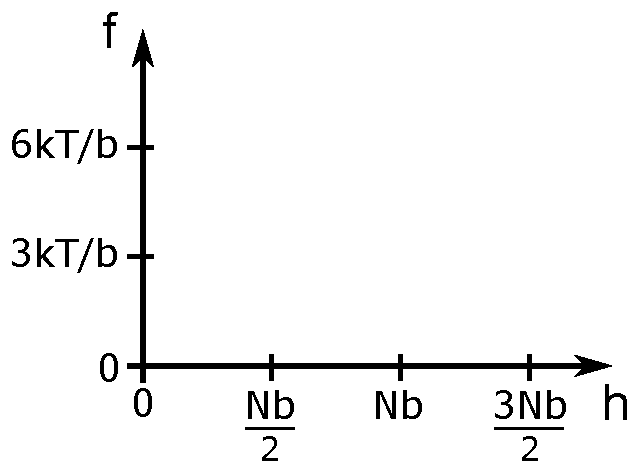
\includegraphics[width=0.5\textwidth]{\figpath/Model2_Fdaxes_blank}}}
			\centerline{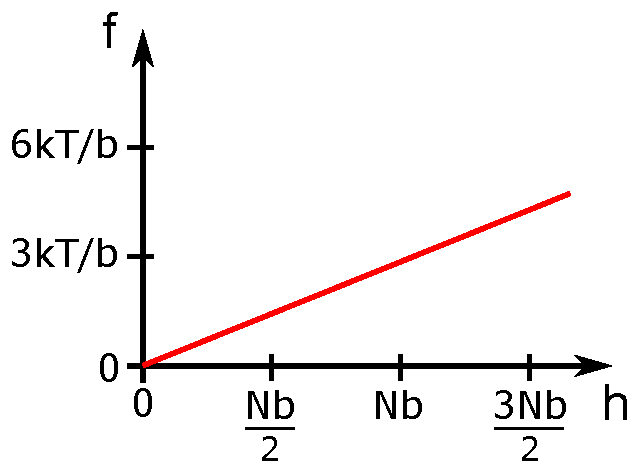
\includegraphics[width=0.5\textwidth]{\figpath/Model2_Fdaxes_gaussian-soln}}
		\end{solution}
		
	\question According to this force-extension relationship, is there anything preventing the chain from being stretched to end-to-end distances larger than $h=Nb$?
	
		\begin{solution}[1.5in]{}
			No.  As shown in this plot, the force keeps increasing linearly with end-to-end distances even when $h > Nb$.  According to this plot, it should be possible to reach end-to-end distances greater than $Nb$ as long as you apply a large enough force.
		\end{solution}
	
	\question If it is \textit{physically impossible} to extend the chain past length $Nb$, what must happen to the force on the chain at this point?  Briefly explain your group's reasoning.
	
		\begin{solution}[1.5in]{}
			The force should diverge to infinity/increase so much that you physically can't pull the chain to a longer length.
		\end{solution}
	
	\question Sketch the force-distance curve you would expect to measure for a ``real'' chain on the axes below: \label{\labelbase:ctq:guessrealFd}
	
		\begin{solution}[2in]{\centerline{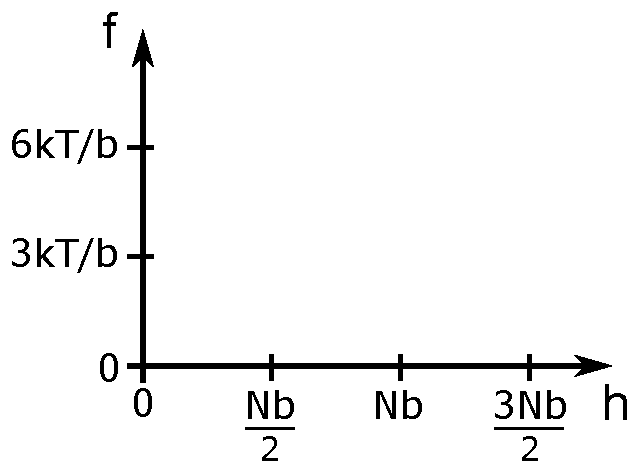
\includegraphics[width=0.5\textwidth]{\figpath/Model2_Fdaxes_blank}}}
			\centerline{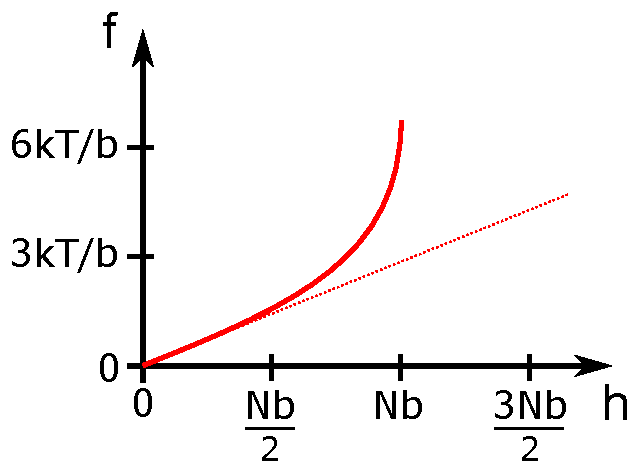
\includegraphics[width=0.5\textwidth]{\figpath/Model2_Fdaxes_realchain-soln}}
		\end{solution}
	
\end{ctqs}

\begin{model}
\label{\labelbase:mdl:langevinchain}

	It is possible to show (see Exercise \ref{\labelbase:exc:langevinderivation}) 
	that the force-distance curve for a freely-jointed chain that cannot be extended past its contour length is more accurately given by
	\begin{equation*}
		f = \frac{k_BT}{b} \mathcal{L}^{-1}\left(\frac{h}{Nb}\right) \label{\labelbase:eqn:Fdlangevin}
	\end{equation*}
	where $\mathcal{L}^{-1}$ is the so-called ``inverse Langevin function''.
	
	The inverse Langevin function has the following shape:
	
	\centerline{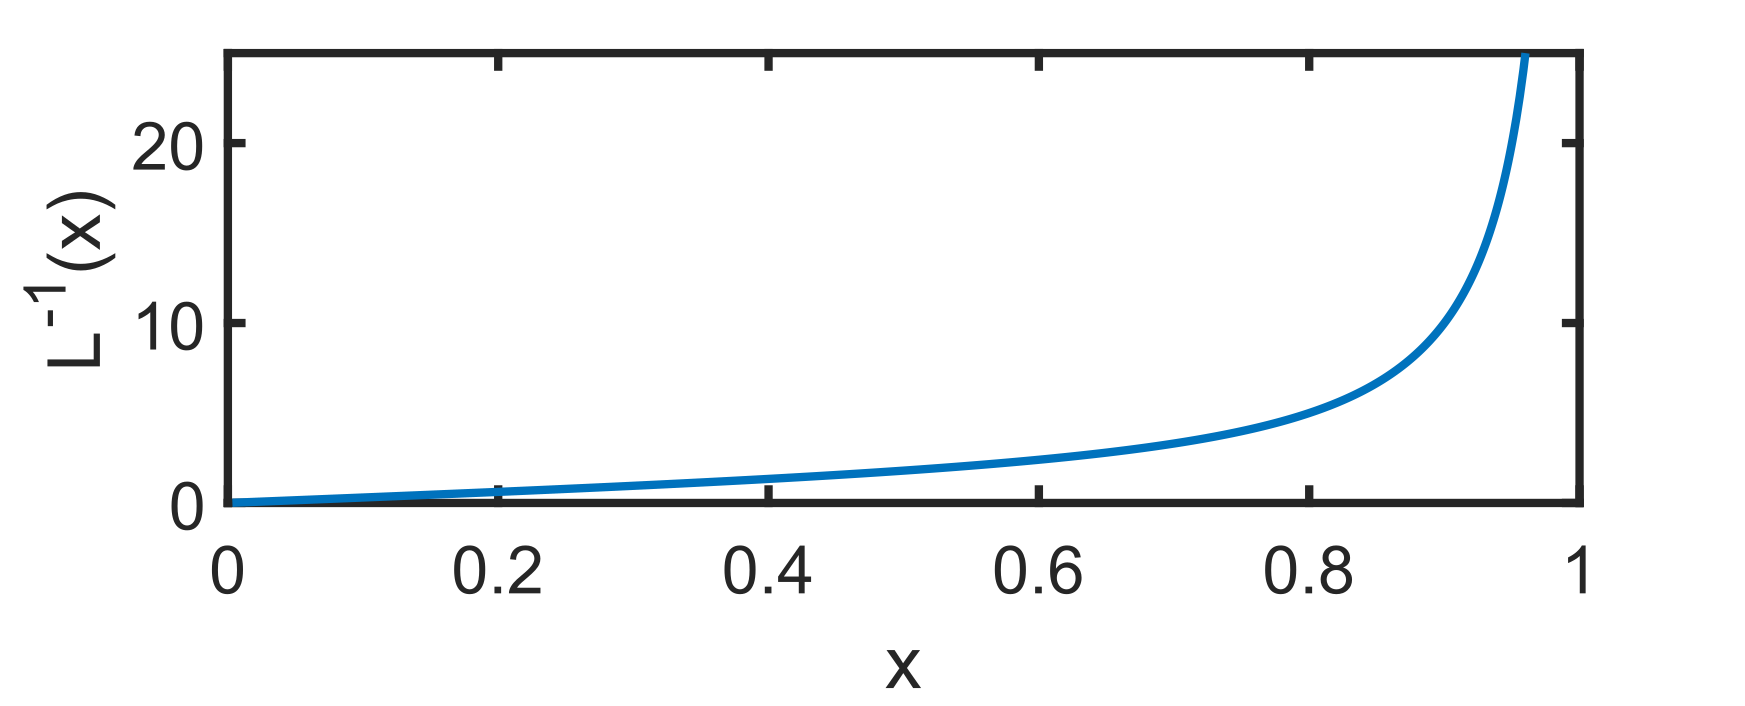
\includegraphics[width=0.5\textwidth]{\figpath/langevin-function.png}}
	
\end{model}

\begin{ctqs}
	
	\question Is this functional form consistent with your answer to CTQ \ref{\labelbase:ctq:guessrealFd}?  If not, sketch a more accurate depiction of the force-distance curve for a ``real'' chain on the axes below:
	
		\begin{solution}[2in]{\centerline{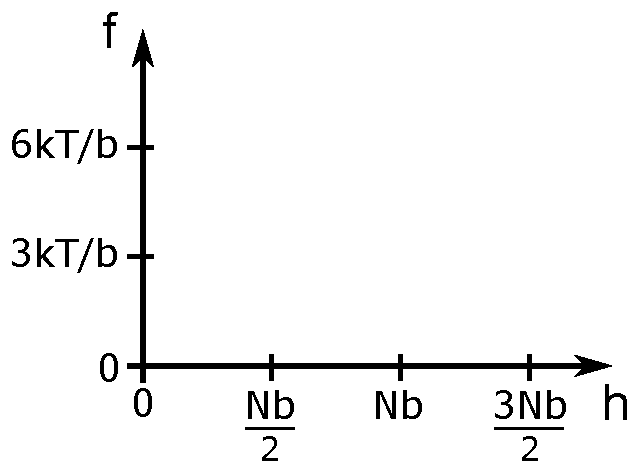
\includegraphics[width=0.5\textwidth]{\figpath/Model2_Fdaxes_blank}}}
			Most students will probably have gotten the right shape in CTQ \ref{\labelbase:ctq:guessrealFd}, but if not, they should sketch this here: 
			
			\centerline{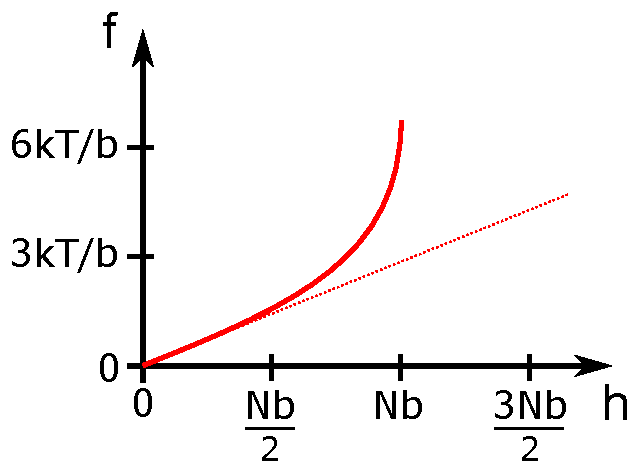
\includegraphics[width=0.4\textwidth]{\figpath/Model2_Fdaxes_realchain-soln}}
		\end{solution}
	
	\question The inverse Langevin function can be approximated using a Taylor series expansion as follows:\footnote{see DOI: 10.1007/s00397-014-0802-2}
		\begin{equation*}
			\mathcal{L}^{-1}(x) = 3x + \frac{9}{5}x^3 + \frac{297}{175}x^5 + \dots
		\end{equation*}
		
		\begin{enumerate}
			\item When $x=\frac{h}{Nb}$ is small (i.e. $x \ll 1$), why is it reasonable to assume that the $x^3$ and $x^5$ terms make a negligible contribution to the measured force?  Briefly explain your group's reasoning.
			
				\begin{solution}[1.5in]{}
					When you take a number that is much less than 1 and take it to the third or fifth power, the value gets even closer to zero (for example, if $x=0.1$, $x^3=0.001$ and $x^5=0.00001$).  The $x^3$ and $x^5$ terms are thus much smaller than the $x$ term, so they don't change the calculated value of $\mathcal{L}^{-1}(x)$, and in turn the force, by very much.
				\end{solution}
			
			\item Using $\mathcal{L}^{-1}(x) \approx 3x$, find an expression for the force on a freely-jointed chain with $N$ links of length $b$ in the low extension limit. \label{\labelbase:ctq:small-h-approx}
			
				\begin{solution}[1.75in]{}
					When $\mathcal{L}^{-1}(x) \approx 3x$, $\mathcal{L}^{-1}(\frac{h}{Nb}) \approx \frac{3h}{Nb}$.  Plugging this into the expression for $f$ given on the previous page,
					\begin{equation*}
						f(x) \approx \frac{k_BT}{b}\left(3\frac{h}{Nb}\right) = \frac{3k_BT}{Nb^2}h
					\end{equation*}
				\end{solution}
			
		\end{enumerate}
		
	\question Compare your answer to the preceding question to the equation given in the information box on page \pageref{\labelbase:info:gaussfd}, and use your observations to critique or defend the following statement in 2-3 complete sentences:
	
		\emph{``The Gaussian distribution offers a reasonable description of the conformations and force responses of polymer chains at low extensions, but fails when chains are stretched to extensions approaching their contour lengths.''}
			
				\begin{solution}[2in]{}
					The expressions for the force given in CTQ \ref{\labelbase:ctq:small-h-approx} and in the information box on page \pageref{\labelbase:info:gaussfd} are the same.  Based on this result, it appears that the Gaussian force law (based on Gaussian chain conformations) does do a reasonable job of describing the conformations and force-extension curve fo the chain as long as $\frac{h}{Nb}$ (the extension of the chain) is small.  As we saw in Model \ref{\labelbase:model:chainstretching} and CTQ \ref{\labelbase:ctq:guessrealFd}, however, the Gaussian prediction fails as $h$ approaches $Nb$ or the chain is stretched to near its contour length.  Thus, the statement in this question appears to be correct.
				\end{solution}
	
\end{ctqs}
	

\begin{exercises}

	%\exercise Propose a method that you could use to measure the force-distance curve for a single polymer chain.
	
	%	\begin{solution}{}
	%		Force-distance curves of a single polymer chain can be measured using an atomic force microscope or optical tweezers.  
	%	\end{solution}
	
	\exercise Briefly explain how you would expect the force-distance relationship for single polymer chains, as discussed in this activity, to influence the stress-strain curve of a cross-linked polymer network.  If you take a rubber band and slowly stretch it as far as you can, do you indeed observe this behavior?
	
		\begin{solution}{}
			\emph{Note: This question should only be assigned \emph{after} students have completed Activity 8.1.}
			
			~
			
			
			As discussed in Activity 8.1, the stress-strain curves of cross-linked polymer networks originate from the force-extension curves of the polymer chains that make up the network.  As such, the force it takes to stretch a crosslinked rubber should increase sharply as the rubber nears its maximum extension, until it is not possible to stretch the piece of rubber any further without breaking it.	Students should indeed observe this behavior if they slowly stretch a rubber band, as long as the rubber band isn't too old/too brittle.
			
			\emph{Note \#2: the math for translating the strain-stiffening behavior of single polymer chains to the strain-stiffening behavior of polymer networks is non-trivial.  If you do want to have students look through this math after completing Activity 8.1, however, section 6.7 of  Treolar's \emph{The Physics of Rubber Elasticity} is a useful reference.}
		\end{solution}
		
	%\exercise Based on the information presented in this activity, is strain-stiffening of polymer chains an entropic effect, or an enthalpic effect?  Explain your reasoning in a short paragraph.
	
	\exercise Poly(methyl methacrylate) has a Kuhn segment length of $b=1.53$~nm and a Kuhn segment mass of $600$~g/mol.
	
		\begin{enumerate}
			\item How much force would it take to extend a 20~kg/mol chain of poly(methyl methacrylate) to end-to-end distances of (i) 20 nm, (ii) 30 nm, (iii) 40 nm, and and (iv) 50 nm at room temperature (298~K)?
			
				\emph{You will probably find it easiest to rewrite the equation given on page \pageref{\labelbase:eqn:Fdlangevin} as $h = Nb\mathcal{L}\left(\frac{fb}{k_B T}\right)$ and solve this problem graphically.  You will also find it useful to know that the Langevin function is $\mathcal{L}(x)= \frac{e^x + e^{-x}}{e^x - e^{-x}} - \frac{1}{x}$.}
			
				\begin{solution}{}
					First, we need to calculate $N$ for the given 20~kg/mol chain of poly(methyl methacrylate):
					\begin{equation*}
						N = \frac{20\text{ kg/mol}}{600\text{ g/mol}} = 33.3
					\end{equation*}
					
					Next, we need to plot $h$ vs $f$ where $f$ and $\mathcal{L}(x)$ have the forms given in the problem.  Using $N=33.3$, $b=1.53$~nm, $k_B=1.380\times 10^{-23}$~J/K, and $T=298$~K, we obtain
					
					\centerline{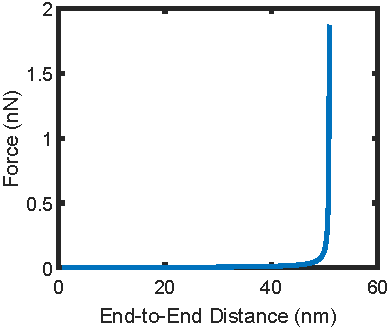
\includegraphics[width=0.5\textwidth]{\figpath/Exc_PMMA_fdsoln}}
					
					Notes about this plot:
					\begin{itemize}
						\item In the calculation used to generate the plot, $f$ was the independent variable, and $h$ was the dependent variable.  However, because the problem is asking about the force as a function of distance, we have plotted the end-to-end distance $h$ on the x axis and the force on the y axis.
						
						\item If your graph does not look like this, check to make sure that you did all of the unit conversions correction - in particular, $b$ must be converted to meters and $f$ must be converted to Newtons for the units to cancel correctly with those in $k_B$ when doing the calculation.
					\end{itemize}
					
					If we zoom in on this plot in the appropriate regions, we can see that the forces required to reach each of the given distances are:
					\begin{center}
						\begin{tabular}{cc}
							\textbf{End-to-End Distance (nm)} & \textbf{Force (nN)} \\\hline
							20 & 0.0035 \\ 
							30 & 0.0062 \\
							40 & 0.0125 \\
							50 & 0.1378 \\
						\end{tabular}
					\end{center}
					
				\end{solution}
			
			\item The force required to break a covalent bond is typically on the order of approximately 1 nN.  Based on this information, at what fraction of its maximum extension do you expect this polymer chain to break?
			
				\begin{solution}{}
					The plot in the previous part of the problem reaches a force of 1~nN at an extension of 50.86~nm.
					
					The contour length of this chain is $Nb = 33.333\times(1.53\text{ nm}) = 51.0$~nm.
					
					Thus, the chain is expected to break at approximately 99.7\% of its maximum extension.
				\end{solution}
				
		\end{enumerate}
		
\exercise
	In Activity 7.1, we learned that the conformations of freely-jointed chains should follow a Gaussian distribution, given by
	\begin{equation*}
		P(N,\vec h_0) = A e^{-\frac{3 h_0^2}{2 N b^2}}
	\end{equation*}
	where $P(N,\vec h_0)$ is the probability of finding a chain with end-to-end vector $\vec h_0$,  $h_0$ is the length of the end-to-end vector (or, distance between the chain ends), and $A$ is a proportionality constant.

	\begin{enumerate} 
	
		\item Using this equation, write down expressions for the probability of finding a chain with $N$ links of length $b$ at each of the following end-to-end distances:
		
			\begin{enumerate}
			
				\item $h_0$ = 0
			
				\begin{solution}{}
					$Ae^{-\frac{3\cdot 0^2}{2Nb^2}} = Ae^0 = A$
				\end{solution}
				
				\item $h_0 = Nb$
			
				\begin{solution}{}
					$Ae^{-\frac{3(Nb)^2}{2Nb^2}} = Ae^{-3N/2}$
				\end{solution}
				
				\item $h_0 = 2Nb$
			
				\begin{solution}{}
					$Ae^{-\frac{3{2Nb}^2}{2Nb^2}} = Ae^{-6N}$
				\end{solution}
				
			\end{enumerate}
			
		\item Are these probabilities consistent with your answer to CTQ \ref{\labelbase:ctq:probgtNb}?  If not, which values disagree?
			
				\begin{solution}{}
					These probabilities are not consistent with the answer to CTQ \ref{\labelbase:ctq:probgtNb}.  In particular, the calculation shows that the probability of finding the chain at an end-to-end distance of $2Nb$ is nonzero.
					
					\emph{Note: numerically, the probabilities of finding the chain as having an end-to-end distance well past $Nb$ are small - for example, when $N=5$ the probability predicted for an end-to-end distance of $2Nb$ is $10^{-13}$ smaller than that of an end-to-end distance of zero - but the key point is that the probabilities are still \emph{nonzero}.}
				\end{solution}

		\end{enumerate}

%
	\exercise \label{\labelbase:exc:langevinderivation} One way to justify the force-extension relationship for the Langevin chain given on page \pageref{\labelbase:eqn:Fdlangevin} is to recognize that as we pull on a chain, we change its internal energy by doing work on the chain, and this in turn changes the probability of finding the chain in each configuration (higher-energy configurations are, from a statistical mechanics perspective, less likely to occur).
	
	Work through this derivation by doing the following:

	\begin{enumerate}
		\item Suppose a chain starts at end-to-end distance $h=0$.  Force $f$ is applied to stretch the chain to end-to-end distance $h=R$.  How much \textit{work} is done on the chain during this process?
		
			\begin{solution}{}
				Work = force $\times$ distance, so the amount of work done is $fR$.
			\end{solution}
			
		\item If the energy of the chain was 0 when $h=0$, what is the energy of the chain when $h=R$?
		
			\begin{solution}{}
				The energy we put in by doing work goes directly into increasing the potential energy of the chain.  The energy of the chain with end-to-end distance $R$ is thus just $fR$.
			\end{solution}
			
		\item In statistical mechanics, the probability of observing a state with energy $U$ is
			\begin{equation*}
				\frac{e^{-U/k_B T}}{Z}
			\end{equation*}
			where $Z$ is the ``partition function'',
			\begin{equation*}
				Z = \sum_\text{all states} e^{-U/k_B T}
			\end{equation*}
			Suggest an expression for the \emph{average} value of $R$, $\langle R \rangle$, that would be measured at a given force $f$.
			
			\emph{Hint: in probability, averages are calculated by multiplying the value that would be measured for a given state by the probability of finding the system in that state, and summing over all possible states.}
			
			\begin{solution}{}
				Per the hint,
				\begin{equation*}
					\langle R \rangle = \frac{1}{Z} \sum_\text{all states} R e^{-U/k_B T}
				\end{equation*}
				Substituting in $U=fR$, we obtain
				\begin{equation*}
					\langle R \rangle = \frac{1}{Z} \sum_\text{all states} R e^{-fR/k_B T}
				\end{equation*}
			\end{solution}
			
		\item It is also possible to show that the Gibbs free energy of a system is related to its partition function by
			\begin{equation*}
				G = -k_B T \ln Z
			\end{equation*}
			Use this information, and your answer to the previous question, to show that the average end-to-end distance of the polymer chain is
			\begin{equation*}
				\langle R \rangle = -\frac{\partial G}{\partial f}
			\end{equation*}
			
			\emph{Hint: first, find an expression for $\frac{\partial Z}{\partial f}$.  Then, use the chain rule to calculate $\frac{\partial G}{\partial f}$ and compare your answer to your result from the previous part.}
			
			\begin{solution}{}
				Following the hint in the question, start by calculating the derivative of $Z$ with respect to $f$:
				\begin{align*}
					\frac{\partial Z}{\partial f} &= \frac{\partial}{\partial f}\left( \sum_\text{all states} e^{-U/k_B T} \right) \\
					&= \frac{\partial}{\partial f}\left( \sum_\text{all states} e^{-\frac{fR}{k_B T}} \right) \\
					&= \sum_\text{all states}\left(\frac{\partial}{\partial f} e^{-\frac{fR}{k_B T}}\right) \\
					&= \sum_\text{all states}\left(\frac{-R}{k_B T} e^{-\frac{fR}{k_B T}}\right) \\
					&= -\frac{1}{k_B T}\sum_\text{all states}R e^{-\frac{fR}{k_B T}}
				\end{align*}
				
				Next, take the derivative of $G$ with respect to $f$:
				\begin{equation*}
					\frac{\partial G}{\partial f} = k_B T \frac{1}{Z} \frac{\partial Z}{\partial F}
				\end{equation*}
				Substituting in our expression for $\frac{\partial Z}{\partial f}$ from above and simplifying, we obtain
				\begin{align*}
					\frac{\partial G}{\partial f} &= k_B T \frac{1}{Z} \left( -\frac{1}{k_B T}\sum_\text{all states}R e^{-\frac{fR}{k_B T}} \right) \\
					&= -\frac{1}{Z}\sum_{all states} R e^{-\frac{fR}{k_B T}}\\
					&= -\langle R \rangle
				\end{align*}
				Thus, $\langle R \rangle = -\frac{\partial G}{\partial f}$ as desired.
			\end{solution}
			
		\item For a freely-jointed chain with $N$ links of length $b$, the partition function turns out to be\footnote{see Section 2.6.2 of \emph{Polymer Physics} by Michael Rubinstein and Ralph Colby}
		\begin{equation*}
			Z = \left[ \frac{2\pi}{fb/k_B T}\left(e^{fb/k_B T} - e^{-fb/k_B T}\right)\right]^N
		\end{equation*}
		Using this information, show that
		\begin{equation*}
			\langle R \rangle = bN\left(\coth \beta - \frac{1}{\beta}\right)
		\end{equation*}
		where
		\begin{equation*}
			\beta = \frac{fb}{k_B T}
		\end{equation*}
		and $\coth(x)$ is the hyperbolic cotangent, given by $\coth(x) = \frac{e^x + e^{-x}}{e^x - e^{-x}}$.
		
		\begin{solution}{}
			First, we calculate $G$:
			\begin{align*}
				G &= -k_B T \ln Z = -k_B T \ln \left[ \frac{2\pi}{fb/k_B T}\left(e^{fb/k_B T} - e^{-fb/k_B T}\right)\right]^N\\
				&= -k_B T N \ln\left[ \frac{2\pi k_B T}{fb}\left(e^{fb/k_B T} - e^{-fb/k_B T}\right)\right]
			\end{align*}
			Next, we take the derivative with respect to f:
			\begin{align*}
				\frac{\partial G}{\partial f} &= -k_B T N \frac{\frac{2\pi k_B T}{fb}\left(\frac{b}{k_B T}e^{fb/k_B T} - \frac{-b}{k_B T}e^{-fb/k_B T}\right) + (\frac{-2\pi k_B T}{f^2b})\left(e^{fb/k_B T} - e^{-fb/k_B T}\right))}{\frac{2\pi k_B T}{fb}\left(e^{fb/k_B T} - e^{-fb/k_B T}\right)}\\
				&= -k_B T N \frac{\frac{2\pi k_B T}{fb}\left(\frac{b}{k_B T}e^{fb/k_B T} - \frac{-b}{k_B T}e^{-fb/k_B T}\right)}{\frac{2\pi k_B T}{fb}\left(e^{fb/k_B T} - e^{-fb/k_B T}\right)}
				+k_B T N \frac{(\frac{-2\pi k_B T}{f^2b})\left(e^{fb/k_B T} - e^{-fb/k_B T}\right))}{\frac{2\pi k_B T}{fb}\left(e^{fb/k_B T} - e^{-fb/k_B T}\right)} \\
				&= - N b \frac{e^{fb/k_B T} + e^{-fb/k_B T}}{e^{fb/k_B T} - e^{-fb/k_B T}}
				+\frac{k_B T N}{f} \\
				&= -Nb\left(\coth\left(\frac{fb}{k_B T}\right) - \frac{k_B T}{f b}\right)\\
				&= -Nb\left(\coth \beta - \frac{1}{\beta}\right)
			\end{align*}
			where $\beta = \frac{fb}{k_B T}$.
			
			Finally,
			\begin{equation*}
				\langle R \rangle = -\frac{\partial G}{\partial f} = Nb\left(\coth\beta - \frac{1}{\beta}\right)
			\end{equation*}
			as desired.
		\end{solution}
		
		
	\end{enumerate}
		
\end{exercises}
	
\end{activity}